% Options for packages loaded elsewhere
\PassOptionsToPackage{unicode}{hyperref}
\PassOptionsToPackage{hyphens}{url}
\PassOptionsToPackage{dvipsnames,svgnames,x11names}{xcolor}
%
\documentclass[
  letterpaper,
  DIV=11,
  numbers=noendperiod]{scrartcl}

\usepackage{amsmath,amssymb}
\usepackage{iftex}
\ifPDFTeX
  \usepackage[T1]{fontenc}
  \usepackage[utf8]{inputenc}
  \usepackage{textcomp} % provide euro and other symbols
\else % if luatex or xetex
  \usepackage{unicode-math}
  \defaultfontfeatures{Scale=MatchLowercase}
  \defaultfontfeatures[\rmfamily]{Ligatures=TeX,Scale=1}
\fi
\usepackage{lmodern}
\ifPDFTeX\else  
    % xetex/luatex font selection
\fi
% Use upquote if available, for straight quotes in verbatim environments
\IfFileExists{upquote.sty}{\usepackage{upquote}}{}
\IfFileExists{microtype.sty}{% use microtype if available
  \usepackage[]{microtype}
  \UseMicrotypeSet[protrusion]{basicmath} % disable protrusion for tt fonts
}{}
\makeatletter
\@ifundefined{KOMAClassName}{% if non-KOMA class
  \IfFileExists{parskip.sty}{%
    \usepackage{parskip}
  }{% else
    \setlength{\parindent}{0pt}
    \setlength{\parskip}{6pt plus 2pt minus 1pt}}
}{% if KOMA class
  \KOMAoptions{parskip=half}}
\makeatother
\usepackage{xcolor}
\setlength{\emergencystretch}{3em} % prevent overfull lines
\setcounter{secnumdepth}{-\maxdimen} % remove section numbering
% Make \paragraph and \subparagraph free-standing
\ifx\paragraph\undefined\else
  \let\oldparagraph\paragraph
  \renewcommand{\paragraph}[1]{\oldparagraph{#1}\mbox{}}
\fi
\ifx\subparagraph\undefined\else
  \let\oldsubparagraph\subparagraph
  \renewcommand{\subparagraph}[1]{\oldsubparagraph{#1}\mbox{}}
\fi


\providecommand{\tightlist}{%
  \setlength{\itemsep}{0pt}\setlength{\parskip}{0pt}}\usepackage{longtable,booktabs,array}
\usepackage{calc} % for calculating minipage widths
% Correct order of tables after \paragraph or \subparagraph
\usepackage{etoolbox}
\makeatletter
\patchcmd\longtable{\par}{\if@noskipsec\mbox{}\fi\par}{}{}
\makeatother
% Allow footnotes in longtable head/foot
\IfFileExists{footnotehyper.sty}{\usepackage{footnotehyper}}{\usepackage{footnote}}
\makesavenoteenv{longtable}
\usepackage{graphicx}
\makeatletter
\def\maxwidth{\ifdim\Gin@nat@width>\linewidth\linewidth\else\Gin@nat@width\fi}
\def\maxheight{\ifdim\Gin@nat@height>\textheight\textheight\else\Gin@nat@height\fi}
\makeatother
% Scale images if necessary, so that they will not overflow the page
% margins by default, and it is still possible to overwrite the defaults
% using explicit options in \includegraphics[width, height, ...]{}
\setkeys{Gin}{width=\maxwidth,height=\maxheight,keepaspectratio}
% Set default figure placement to htbp
\makeatletter
\def\fps@figure{htbp}
\makeatother

\usepackage{booktabs}
\usepackage{longtable}
\usepackage{array}
\usepackage{multirow}
\usepackage{wrapfig}
\usepackage{float}
\usepackage{colortbl}
\usepackage{pdflscape}
\usepackage{tabu}
\usepackage{threeparttable}
\usepackage{threeparttablex}
\usepackage[normalem]{ulem}
\usepackage{makecell}
\usepackage{xcolor}
\KOMAoption{captions}{tableheading}
\makeatletter
\@ifpackageloaded{caption}{}{\usepackage{caption}}
\AtBeginDocument{%
\ifdefined\contentsname
  \renewcommand*\contentsname{Table of contents}
\else
  \newcommand\contentsname{Table of contents}
\fi
\ifdefined\listfigurename
  \renewcommand*\listfigurename{List of Figures}
\else
  \newcommand\listfigurename{List of Figures}
\fi
\ifdefined\listtablename
  \renewcommand*\listtablename{List of Tables}
\else
  \newcommand\listtablename{List of Tables}
\fi
\ifdefined\figurename
  \renewcommand*\figurename{Figure}
\else
  \newcommand\figurename{Figure}
\fi
\ifdefined\tablename
  \renewcommand*\tablename{Table}
\else
  \newcommand\tablename{Table}
\fi
}
\@ifpackageloaded{float}{}{\usepackage{float}}
\floatstyle{ruled}
\@ifundefined{c@chapter}{\newfloat{codelisting}{h}{lop}}{\newfloat{codelisting}{h}{lop}[chapter]}
\floatname{codelisting}{Listing}
\newcommand*\listoflistings{\listof{codelisting}{List of Listings}}
\makeatother
\makeatletter
\makeatother
\makeatletter
\@ifpackageloaded{caption}{}{\usepackage{caption}}
\@ifpackageloaded{subcaption}{}{\usepackage{subcaption}}
\makeatother
\ifLuaTeX
  \usepackage{selnolig}  % disable illegal ligatures
\fi
\IfFileExists{bookmark.sty}{\usepackage{bookmark}}{\usepackage{hyperref}}
\IfFileExists{xurl.sty}{\usepackage{xurl}}{} % add URL line breaks if available
\urlstyle{same} % disable monospaced font for URLs
\hypersetup{
  pdftitle={Tidycomm-tests},
  colorlinks=true,
  linkcolor={blue},
  filecolor={Maroon},
  citecolor={Blue},
  urlcolor={Blue},
  pdfcreator={LaTeX via pandoc}}

\title{Tidycomm-tests}
\author{}
\date{}

\begin{document}
\maketitle
\section{Regressionsanalyse mit den Daten ``World of
Journalism''}\label{regressionsanalyse-mit-den-daten-world-of-journalism}

Es ist immer ratsam sich zunächst die Regressionskoeffizienten genau
anzuschauen, was mit einer Tabelle praktisch am besten geht, wie sie in
einsehbar ist.

\begin{table}

\caption{\label{tbl-planets}Planets}

\centering{

\begin{table}

\caption{\label{tab:tbl-planets}Regressionsmodell 1: "Autonomy Selection"}
\centering
\begin{threeparttable}
\begin{tabular}[t]{lrrrrrrr}
\toprule
Variable & B & SE B & beta & t & p & VIF & TOL\\
\midrule
(Intercept) & 3.52 & 0.09 & --- & 38.83 & <.001 & --- & ---\\
work\_experience & 0.01 & 0.00 & .160 & 5.72 & <.001 & 1.01 & .990\\
trust\_government & 0.05 & 0.03 & .050 & 1.85 & .060 & 1.01 & .990\\
\bottomrule
\end{tabular}
\begin{tablenotes}
\item footers
\end{tablenotes}
\end{threeparttable}
\end{table}

}

\end{table}%

\subsection{Analyse der
Voraussetzungen}\label{analyse-der-voraussetzungen}

In der Abbildung Figure~\ref{fig-reslev} ist gut zu erkennen.

\begin{figure}[H]

\centering{

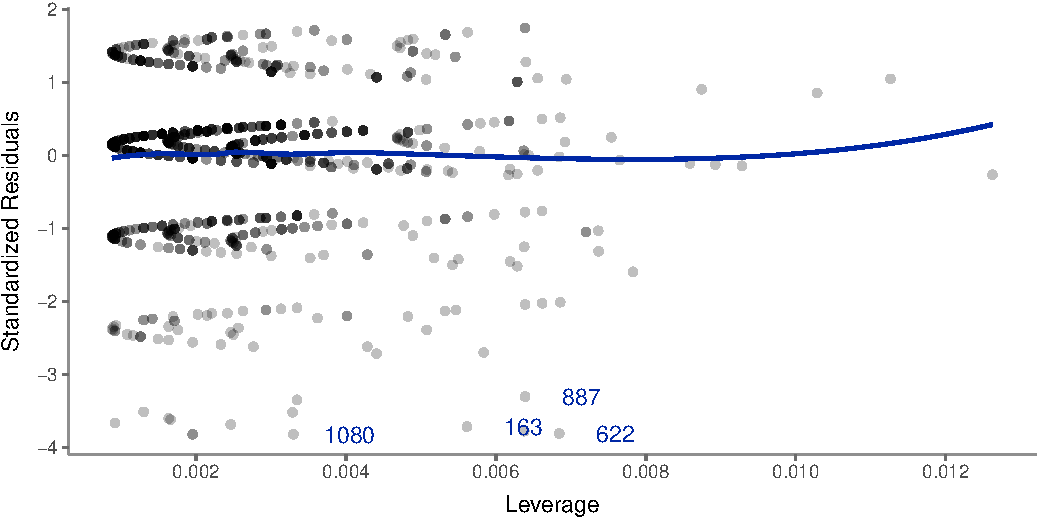
\includegraphics[width=0.85\textwidth,height=\textheight]{testthat_files/figure-pdf/fig-reslev-1.pdf}

}

\caption{\label{fig-reslev}residualsleverage plot}

\end{figure}%

Schaut man sich darüber hinaus Figure~\ref{fig-scaleloc} im schönen
UZH-Design an, wird einem alles klar.

\begin{figure}[H]

\centering{

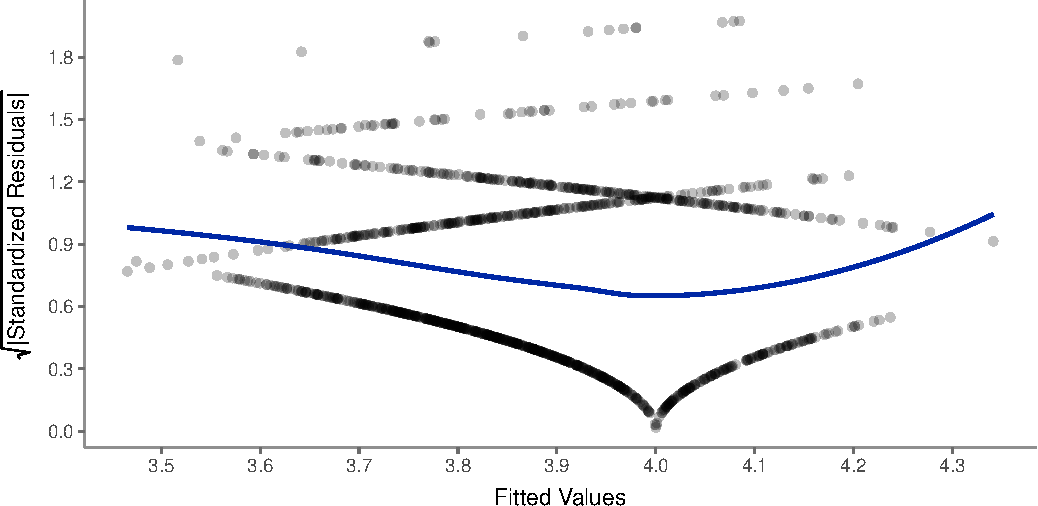
\includegraphics[width=0.85\textwidth,height=\textheight]{testthat_files/figure-pdf/fig-scaleloc-1.pdf}

}

\caption{\label{fig-scaleloc}scalelocation plot}

\end{figure}%

Nicht zuletzt sollte man sich die Residuen in Abhängigkeit der
geschätzten Werte ansehen, was im schönen Viridis-Design in
Figure~\ref{fig-resfit} durchaus möglich ist, auch wenn das dunkle Lila
nicht gut zu erkennen ist.

\begin{figure}[H]

\centering{

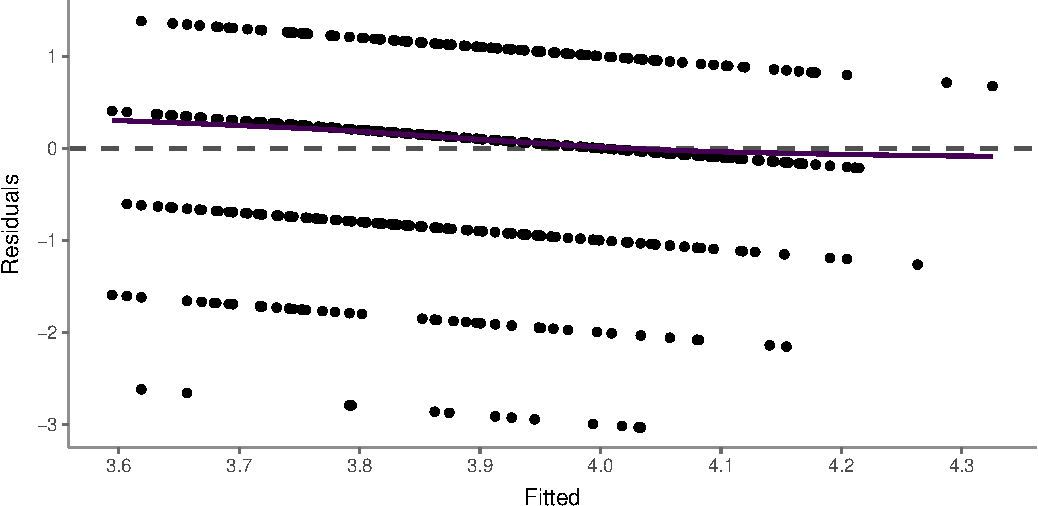
\includegraphics[width=0.85\textwidth,height=\textheight]{testthat_files/figure-pdf/fig-resfit-1.pdf}

}

\caption{\label{fig-resfit}residualsleverage plot}

\end{figure}%



\end{document}
